\documentclass{standalone}
\usepackage{tikz}
\usetikzlibrary{positioning, circuits.ee.IEC, arrows, decorations.pathreplacing}

\begin{document}
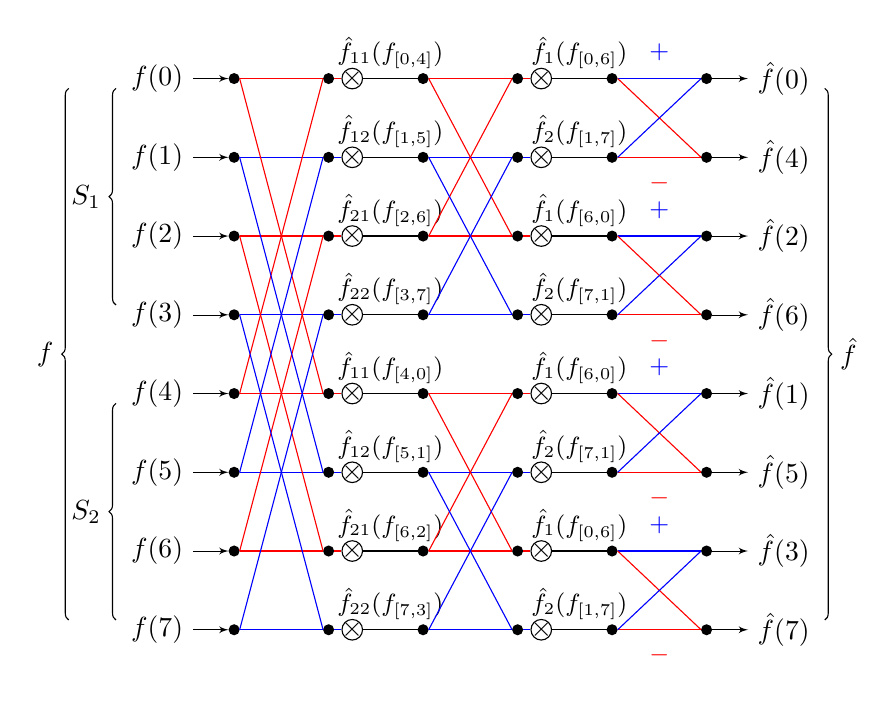
\begin{tikzpicture}
[
    yscale=1.0, xscale=1.2, node distance=0.3cm, auto,
    % The strategy is to create nodes with names: N-column-row
    % Input nodes are named N-0-0 ... N-0-7
    % Output nodes are named N-8-0 ... N-8-5
    circuit ee IEC
]

%=================================== Start ===================================
\tikzstyle{n}   = [circle, fill, minimum size=4pt,inner sep=0pt, outer sep=0pt]
\tikzstyle{mul} = [circle, draw, inner sep=-1pt]
\tikzstyle{box} = [
    draw, align=center, shape=rectangle, minimum width=1.5cm, minimum height=3.5cm,
    append after command={
        % see also: https://tex.stackexchange.com/a/129668
        \foreach \side in {east, west} {
            \foreach \i in {1,...,#1} {
            %  oordinate (\tikzlastnode-\i-\side)
            %  at ($(\tikzlastnode.north \side)!{(\i-.5)/(#1)}!(\tikzlastnode.south \side)$)
                (\tikzlastnode.north \side) edge[draw=none, line to]
                    coordinate[pos=(\i-.5)/(#1)] (\tikzlastnode-\i-\side) (\tikzlastnode.south \side)
            }
        }
    }
]

% Define two helper counters
\newcounter{x} \newcounter{y}
{
    % \node[box=4] (box-t) {$N = \frac{T}{2}$ \\\\ DFT};
    % \node[box=4, below=of box-t] (box-b) {$N = \frac{T}{2}$ \\\\ DFT};

    % Draw groups: Source
    \foreach \y in {0,...,7}
        \node (S-\y) at (-1.25,-\y) {};
    \draw[decorate, decoration={brace,mirror}] (S-0) -- node[left=2pt] {$S_1$} (S-3);
    \draw[decorate, decoration={brace,mirror}] (S-4) -- node[left=2pt] {$S_2$} (S-7);
    \foreach \y in {0,...,7}
        \node (S-\y) at (-1.75,-\y) {};
    \draw[decorate, decoration={brace,mirror}, ] (S-0) -- node[left=2pt] {$f$} (S-7);

    % Draw groups: Result
    \foreach \y in {0,...,7}
        \node (S-\y) at (6.25,-\y) {};
    \draw[decorate, decoration={brace}] (S-0) -- node[right=2pt] {$\hat{f}$} (S-7);
    

    % Draw inputs
    \foreach \y \i \g in {0/0/0, 1/2/1, 2/4/2, 3/6/3, 4/1/0, 5/3/1, 6/5/2, 7/7/3}
        \node[n, pin={[pin edge={latex'-,black}]left:$f(\y)$}]
              (N-0-\y) at (0,-\y) {};
    % Draw outputs
    \foreach \y / \idx in {0/0, 1/4, 2/2, 3/6,
                           4/1, 5/5, 6/3, 7/7}
        \node[n, pin={[pin edge={-latex',black}]right:$\hat{f}(\idx)$}]
              (N-7-\y) at (5,-\y) {};
   % draw connector nodes
    \foreach \y in {0,...,7}
        \foreach \x / \c in {1/1, 2/3, 3/4, 4/6}
            \node[n, name=N-\c-\y] at (\x,-\y) {};
    % draw x nodes
    \foreach \y in {0,...,7}
        \foreach \x / \c  in {1/2,4/5}
            \node[mul, right of=N-\x-\y] (N-\c-\y) {${\times}$};
    
    % horizontal connections
    % Note the use of simple counter arithmetics to get correct
    % indexes.
    \foreach \x in {0,1,3,4}{
        \foreach \y in {0,2,4,6}
        {
            \setcounter{x}{\x}\stepcounter{x}
            \path (N-\x-\y) edge[-,red] (N-\arabic{x}-\y);
        }
        \foreach \y in {1,3,5,7}
        {
            \setcounter{x}{\x}\stepcounter{x}
            \path (N-\x-\y) edge[-,blue] (N-\arabic{x}-\y);
        }
    }
    \foreach \x in {6}{
        \foreach \y in {0,2,4,6}
        {
            \setcounter{x}{\x}\stepcounter{x}
            \path (N-\x-\y) edge[-,blue] (N-\arabic{x}-\y);
        }
        \foreach \y in {1,3,5,7}
        {
            \setcounter{x}{\x}\stepcounter{x}
            \path (N-\x-\y) edge[-,red] (N-\arabic{x}-\y);
        }
    }
    % Draw the W_8 coefficients
    \setcounter{y}{0}
    \foreach \i / \j / \p in {11/f_{[0,4]}, 12/f_{[1,5]}, 21/f_{[2,6]}, 22/f_{[3,7]}, 
                              11/f_{[4,0]}, 12/f_{[5,1]}, 21/f_{[6,2]}, 22/f_{[7,3]}} 
    {
        \path (N-2-\arabic{y}) edge[-] node {\small $\hat{f}_{\i} (\j)$}
              (N-3-\arabic{y});
        \addtocounter{y}{1}
    }
    % Draw the W_4 coefficients
    \setcounter{y}{0}
    \foreach \i / \j / \p in {1/f_{[0,6]}/[0], 2/f_{[1,7]}/[0], 1/f_{[6,0]}/[4], 2/f_{[7,1]}/[2], 
                              1/f_{[6,0]}/[2], 2/f_{[7,1]}/[1], 1/f_{[0,6]}/[6], 2/f_{[1,7]}/[3]}
    {
        \path (N-5-\arabic{y}) edge[-] node {\small $\hat{f}_{\i} (\j)$}
              (N-6-\arabic{y});
        \stepcounter{y}
    }
    % Connect nodes
    \foreach \sourcey / \desty in {0/4, 2/6, 4/0, 6/2}
       \path (N-0-\sourcey.east) edge[-,red] (N-1-\desty.west);
    \foreach \sourcey / \desty in {1/5, 3/7, 5/1, 7/3}
       \path (N-0-\sourcey.east) edge[-,blue] (N-1-\desty.west);
    \foreach \sourcey / \desty in {0/2, 2/0, 4/6, 6/4}
        \path (N-3-\sourcey.east) edge[-,red] (N-4-\desty.west);
    \foreach \sourcey / \desty in {1/3, 3/1, 5/7, 7/5}
        \path (N-3-\sourcey.east) edge[-,blue] (N-4-\desty.west);
    \foreach \sourcey / \desty in {0/1, 2/3}
        \path (N-6-\sourcey.east) edge[-,red] node[right = 17pt, below = 17pt] 
                {\small $-$} 
              (N-7-\desty.west);
    \foreach \sourcey / \desty in {4/5, 6/7}
        \path (N-6-\sourcey.east) edge[-,red] node[right = 17pt, below = 17pt]
                {\small $-$} 
              (N-7-\desty.west);
    \foreach \sourcey / \desty in {1/0, 3/2}
        \path (N-6-\sourcey.east) edge[-,blue] node[right = 17pt, above = 17pt] 
                {\small $+$} 
              (N-7-\desty.west);
    \foreach \sourcey / \desty in {5/4, 7/6}
        \path (N-6-\sourcey.east) edge[-,blue] node[right = 17pt, above = 17pt] 
                {\small $+$} 
              (N-7-\desty.west);
}
%==================================== END ====================================

\end{tikzpicture}
\end{document}